\documentclass[10pt, compress]{beamer}
\usetheme[conference=Preparation,venue=Remote, date=31/13/2017, titleprogressbar, logo=RFX-logo]{Eurof}
\usepackage{listings,amsmath,multimedia, amssymb}
\usepackage{tangocolors}
\usepackage{rfxcolor}
% for drawing
\usepackage{pgf}
\usepackage{tikz}
\usetikzlibrary{arrows,shapes,backgrounds}
\usepackage{onimage}
\usepackage[export]{adjustbox}
\usepackage{bm}
% for font
\usepackage[absolute,overlay]{textpos}
  \setlength{\TPHorizModule}{1mm}
  \setlength{\TPVertModule}{1mm}

\usepackage[style=nature,citestyle=authoryear-comp,defernumbers=true,maxnames=2,firstinits=true,
uniquename=init,backend=bibtex8,arxiv=abs,mcite]{biblatex}
\bibliography{biblio}
\renewcommand*{\bibfont}{\footnotesize}
\renewcommand*{\citesetup}{\footnotesize}
\usepackage[export]{adjustbox}
\makeatother
\mode<presentation>
\makeatletter
% add a macro that saves its argument
\newcommand{\footlineextra}[1]{\gdef\insertfootlineextra{#1}}
\newbox\footlineextrabox
% for reducing font on a single slide
\newcommand\Fontvi{\fontsize{8}{7.2}\selectfont}
\title{Topic 21: Week 17 Experimental preparation}
\date{31 March 2017}
\author[Topic 21]{Topic 21 ST}
\begin{document}
\tikzstyle{every picture}+=[remember picture]
\maketitle
\section{L-Mode}
\begin{frame}{Current scan at constant q$_{95}$}
  \vspace{-1cm}
  \Fontvi
  \centering{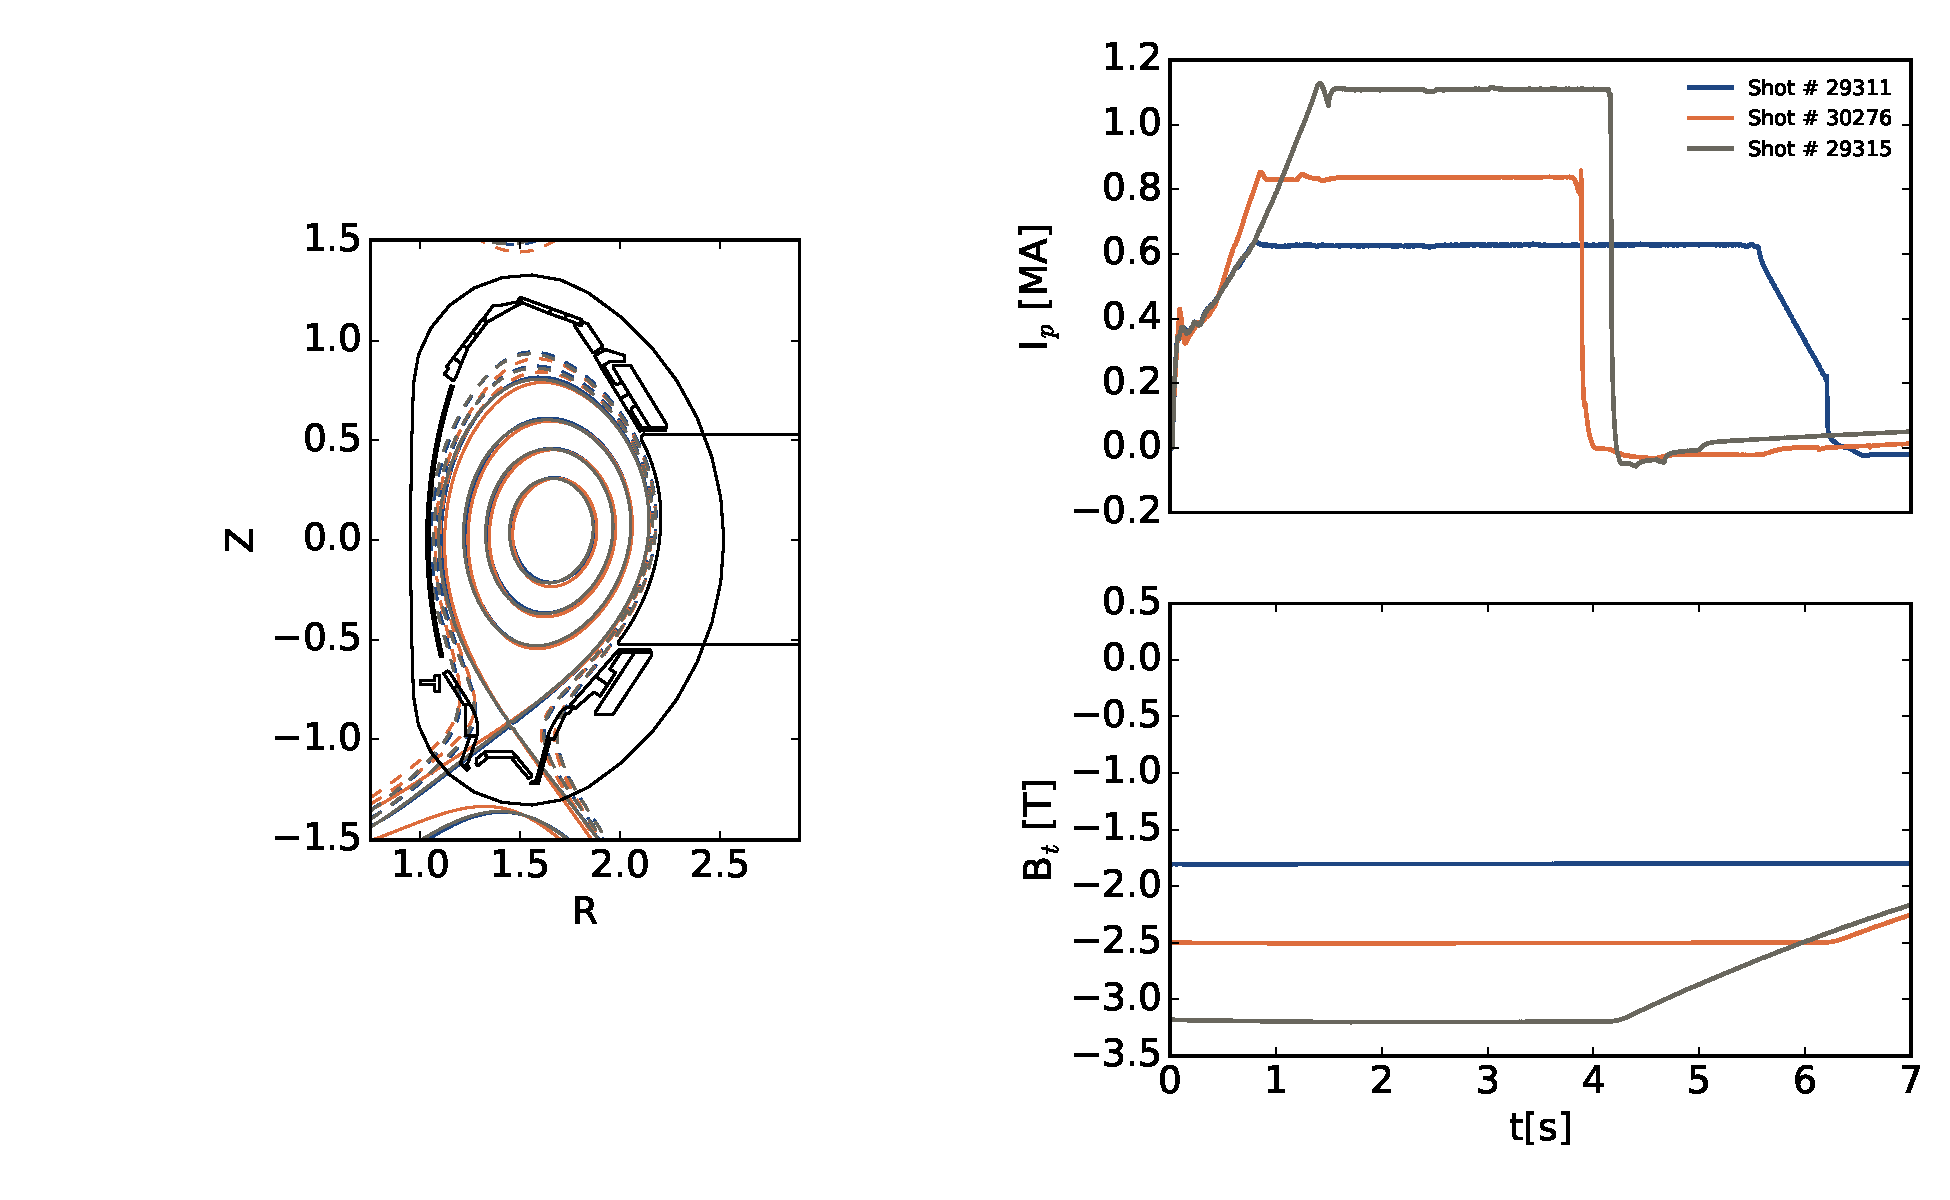
\includegraphics[width=0.85\textwidth]{../analysis/pdfbox/CurrentScanConstantQ95}}
  \begin{itemize}
    \item The shot at lower and higher current has NBI which need to
      be substituted with ECRH (I guess the amount used in \# 30269 is
      sufficent)
    \item The fueling rate needs to be adjusted for lower current in
      order not to disrupt to early
    \item The higher current (it is the only reference I have for 1MA
      with this value of q$_{95}$) encounter an early
      disruption. \alert{Contact SL in order to check and avoid the reason}
  \end{itemize}    
\end{frame}

\begin{frame}{Current scan at constant B$_t$}
  \Fontvi
  \centering{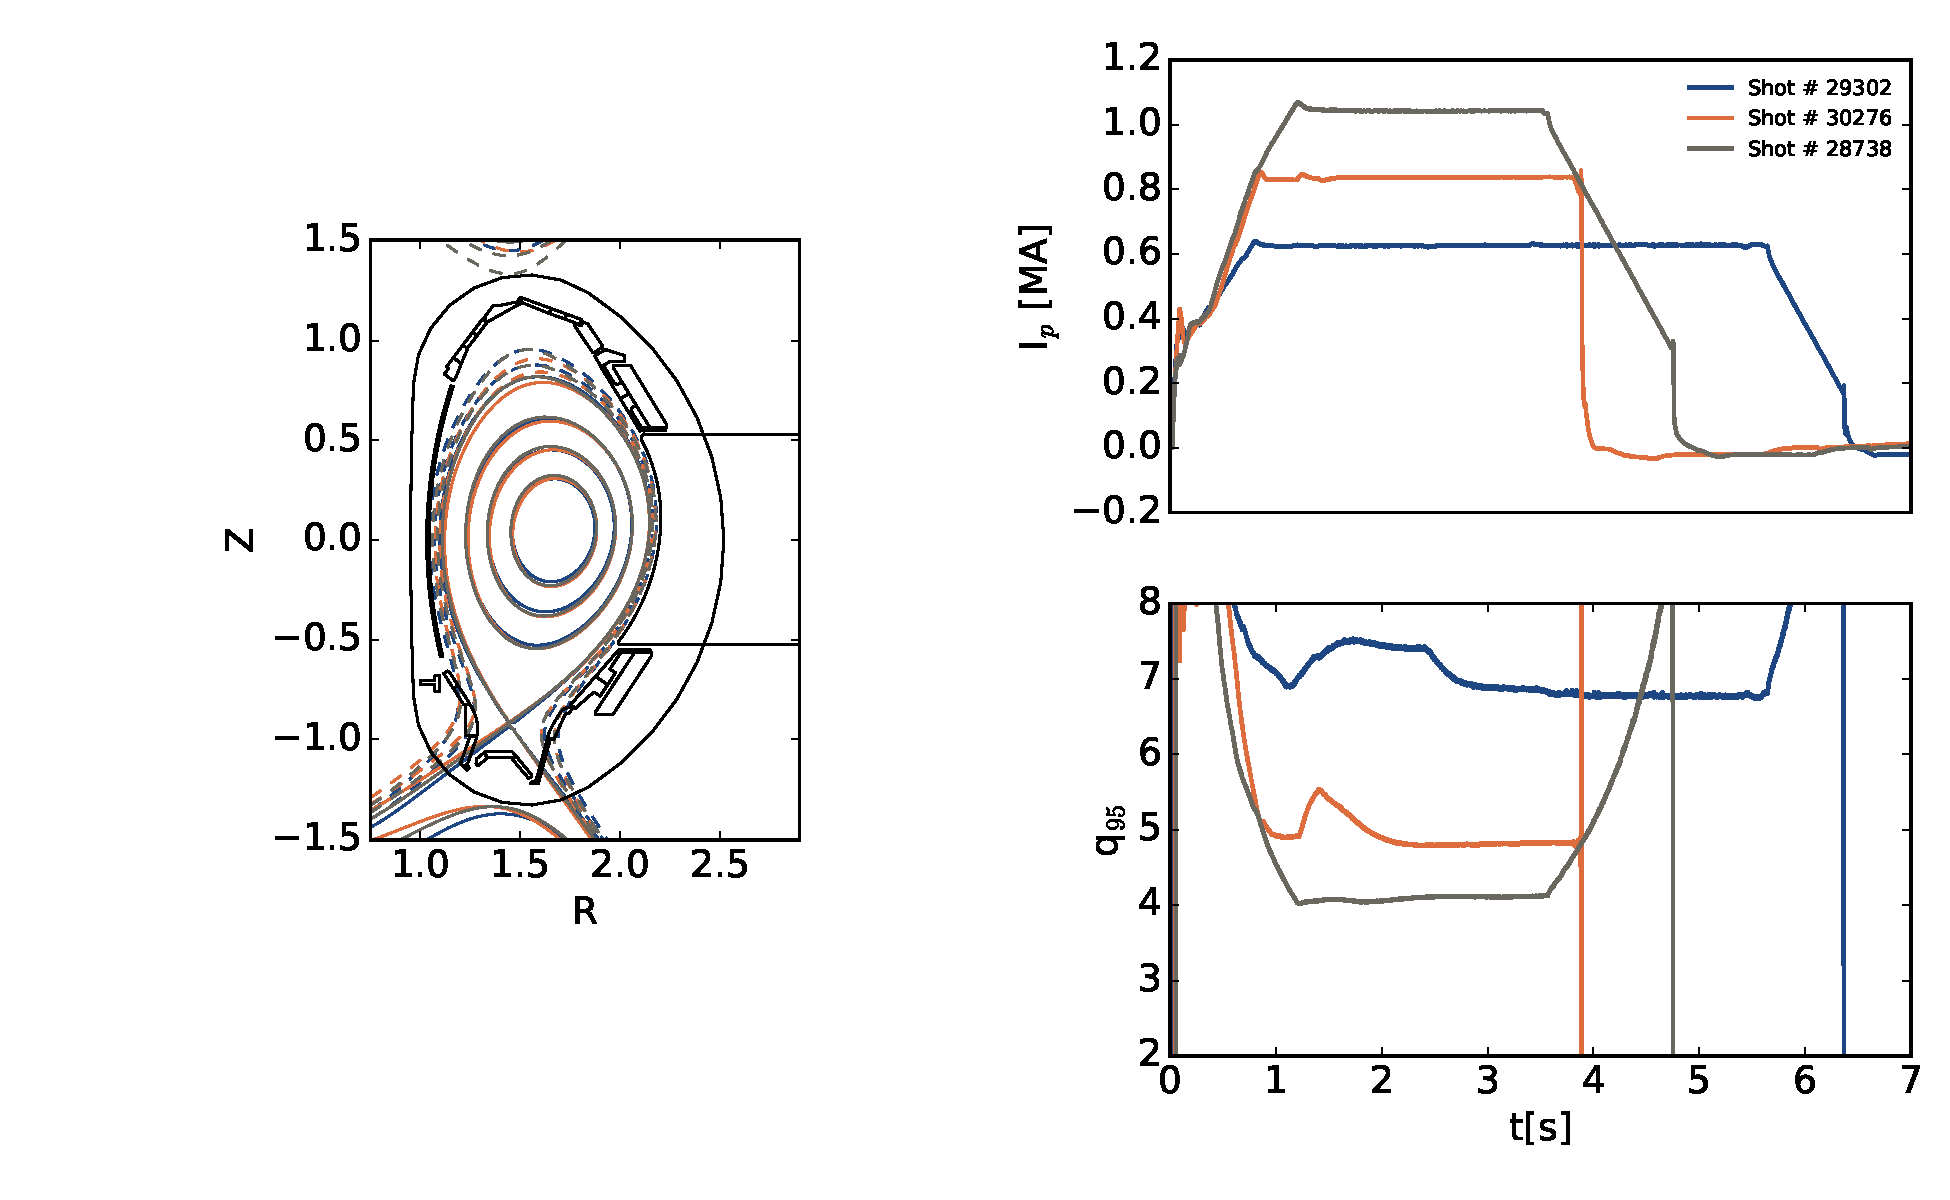
\includegraphics[width=0.85\textwidth]{../analysis/pdfbox/CurrentScanConstantBT}}
  \begin{itemize}
    \item We have a slightly different upper triangularity for the
      reference shot. \alert{Is this an issue?}
    \item The fueling rate needs to be adjusted for lower current in
      order not to disrupt to early
  \end{itemize}    
\end{frame}


\begin{frame}{Shot list: L-Mode}
  \begin{enumerate}
    \item Repeat \# 23902, with fuelling rate reduced with respect to
      \# 30269 by 20\%. No NBI, 300 kW (\alert{Sufficient? shall we increase?}) ECRH central heating.
    \item Repeat \# 29311 with the same fuelling rate and heating as
      the previous. Should be fine for Reflectometer measurements
    \item Repeat \# 28738 with 300 kW ECRH central heating and same
      fueling as reference
    \item Repeat \# 29315 with correction in order to avoid disruption
  \end{enumerate}
  \end{frame}
  \section{H-Mode}
  \begin{frame}{H-Mode reference}
\vspace{-1cm}
    \Fontvi
  \centering{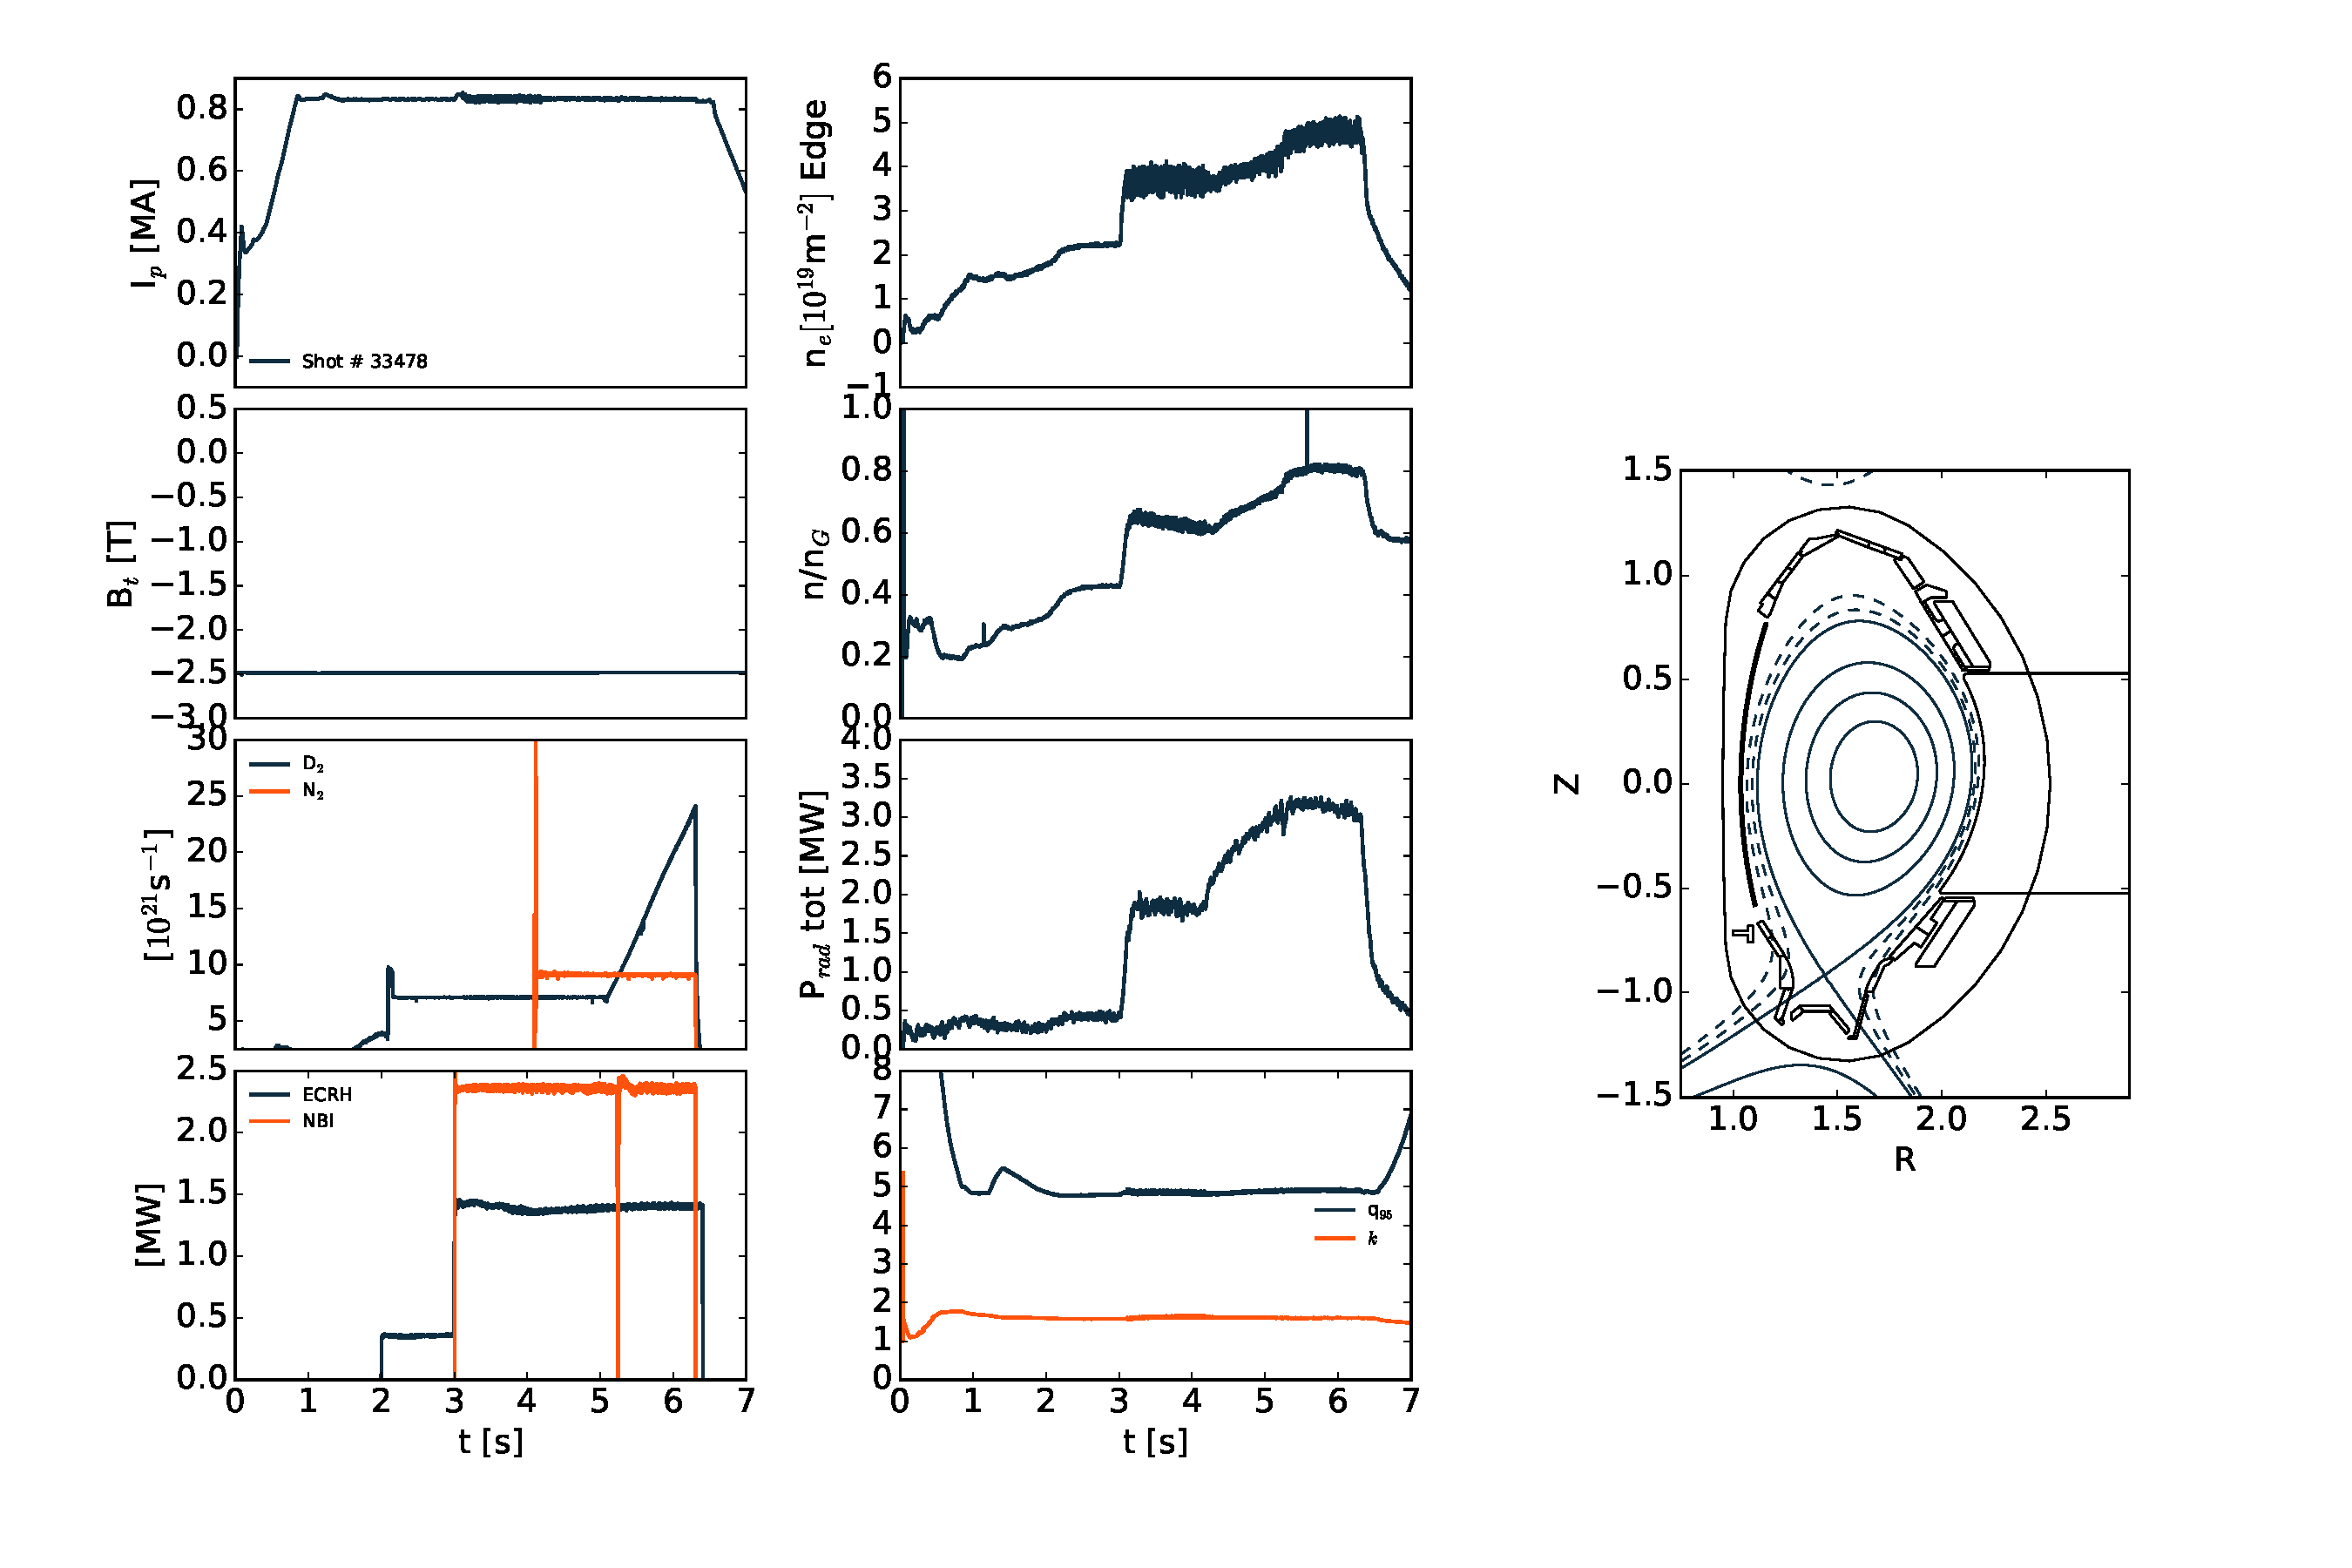
\includegraphics[width=0.85\textwidth]{../analysis/pdfbox/ReferenceHMode}}
  \begin{itemize}
    \item This should be the best reference mode we have from last year
    \item We should run this shot with P$_{NBI}\approx $4MW
    \item I'm not sure we can increase further the fueling since we
      already reach $n/n_G\approx 0.8$. Eventually we can start
      earlier and reduce the rate a bit
  \end{itemize}    
  \end{frame}
  \begin{frame}{H-Mode list}
    \begin{enumerate}
      \item Repeat \# 33478 with P$_{NBI}$ = 4MW and without seeding. Start D$_2$
        puffing earlier @ 4s reaching 25$\times 10^{21}$ @
        6s. Plunge of probe head at 5.2s.
        \item Repeat \#1 eventually with modification to fueling
          Add seeding in feed-forward as in reference shot. Plunge of
          the probe head @ 5.2 s
        \item Trade off between \#1 and \#2. If the probe does not
          exhibit problem 2 plunges @4.8 and 5.6
    \end{enumerate}
  \end{frame}
  \begin{frame}{To be done}
  \begin{itemize}
    \item[$\square$] Contact Reference Session Leader. E. Wolfrum (?)
    \item[$\square$] Check consistency of the equilibria in term of
      SOL field line. \alert{seems reasonable}
    \item[$\square$] Together with reference session leader check \#
      29315 for early disruption
    \item[$\square$] Prepare analysis tools for inter-shot evaluation
    \item[$\square$] Camera for neutral profile has been
      calibrated. Contact for CAD and field line tracing
    \item[$\square$] Check presence of relevant people in control room
      for operation of Bolometer/SXR/Langmuir/Gauges
    \item[$\square$] Prepare a task list for control room. We need
      people evaluating data on the fly
  \end{itemize}
\end{frame}

\end{document}

